\chapter{Enabling Technologies}
\label{chap:entech}


In this chapter, the technologies used to achieve this projects' objective shall be discussed.

\section{Introduction}\par
In this project two main technologies have been used:~\acf{nlp}  and~\acf{ml}. The implementation of these tools has been performed in a combined fashion. Furthermore, other technologies have also been used but they are less relevant than~\ac{nlp} and~\ac{ml}.
On the one hand, with~\ac{nlp} it was possible to transform words into tokens, find syntactical connections between tokens in the same tweet and, finally, construct a numerical vector. On the other hand,~\ac{ml} was very useful to construct a classifier, define a model and feed the vectors from the previous step into the model to make predictions.\par
In short, this is how the project was carried out. Both technologies will be extensively explained in the next sections.

\section{Natural Language Processing}
\ac{nlp} has a crucial role in this project since texts (tweets) is what this project is trying to deal with. Hence, the information that used to train the~\ac{ml} algorithm will come in the form of text. According to~\cite{bird2009natural}, at one extreme~\ac{nlp} could be as simple as counting word frequencies to compare different writing styles. At the other extreme,~\ac{nlp} involves "understanding" complete human utterances, at least to the extent of being able to give useful responses to them.\\
\begin{figure}
	\hspace{-1.45cm}
	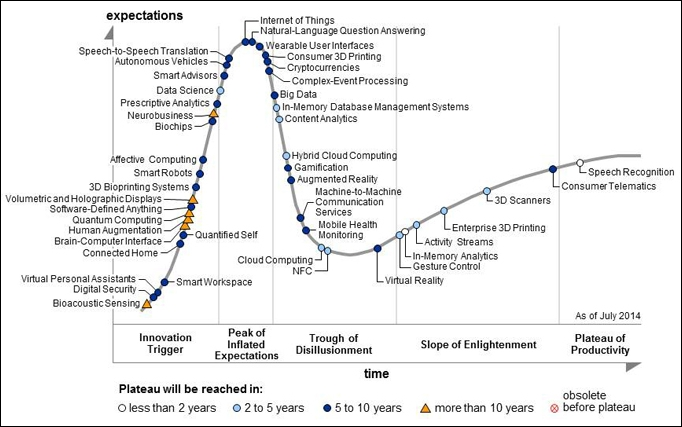
\includegraphics[]{img/nlp.jpg}
	\caption{Image is taken from~\url{http://www.gartner.com/newsroom/id/2819918}}
	\label{fig:nlptech}
\end{figure}
When the task is handling text,~\ac{nlp} is a very powerful tool. Such is the importance that many other applications that can be found everyday already implement it. \Cref{fig:nlptech} shows many emerging technologies that are using \ac{nlp} to provide their services.
Many other examples of \ac{nlp} applications are machine translation, optical character recognition, language detection, topic modelling and many more~\cite{stopwords}.

\label{sec:NLP}
\subsection{Natural Language Toolkit}
\subsubsection{Definition}
\ac{nltk} is a platform for building Python programs to work with human language data. It provides easy-to-use interfaces to over 50 corpora and lexical resources such as WordNet, along with a suite of text processing libraries for classification, tokenization, stemming, tagging, parsing, and semantic reasoning, wrappers for industrial-strength~\ac{nlp} libraries, and an active discussion forum~\footnote{https://www.nltk.org/}.\\
The following applications explained beneath belong to the~\ac{nltk} class.
\subsubsection{Application}
~\ac{nltk} has provided the following tools to this project:
\begin{itemize}
	
	\item \textit{Tokenizer}: A word (Token) is the minimal unit that a machine can understand and process. So any text string cannot be further processed without going through tokenization. Tokenization is the process of splitting the raw string into meaningful tokens~\cite{nltk}. In this project, tokenization was required to get the words containing a tweet. Furthermore, some of the tokens were removed since they do not add meaningful information (e.g. yo, a). These words belong to a stoplist provided by~\ac{nltk} for all supported languages~\cite{nltk}.
	\item \textit{Stemmer}: A stemmer is needed to remove affixes from a word, ending up with a stem. Stemming is frequently used for indexing words. Instead of storing all forms of a word, the algorithm stores only the stems, greatly reducing the size of the index while increasing retrieval accuracy~\cite{nltk}. Particularly, the SnowballStemmer was chosen because it supports stemming in 13 non-English languages, especially Spanish.
	\item \textit{Part-of-Speech tagging}:  A-part-of-Speech tagger (pos\_tag) indicates how a word is functioning within the context of a sentence~\cite{pos}. This part is crucial since a word can function in multiple ways and we would like to distinguish those cases. POS\_tagging has been achieved by collecting each word feature and building up a dictionary with the word features' stats. The word features offered by~\ac{nltk} are:
	\begin{enumerate}
		\item \textit{VERB}: Verbs (all tenses and modes)
		\item \textit{NOUN}: Nouns (common and proper)
		\item \textit{PRON}: Pronouns
		\item \textit{ADJ}: Adjectives
		\item \textit{ADV}: Adverbs
		\item \textit{ADP}: Adpositions (prepositions and postpositions)
		\item \textit{CONJ}: Conjunctions
		\item \textit{DET}: Determiners
		\item \textit{NUM}: Cardinal numbers
		\item \textit{PRT}: Particles or other function words
		\item \textit{X-other}: Foreign words, typos, abbreviations
		\item \textit{.}: Punctuation
	\end{enumerate}
\end{itemize}

The applications at the top of this section are more commonly known as the preprocessing part previously needed to any \ac{ml} application. Since there are plenty of tasks, they could be easily coordinated by using pipelines.\\ 
More information on how were these technologies implemented in the project can be found in~\cref{sec:preprocessing}.

\section{Machine Learning}
When it comes to defining models capable of learning from a text-based source, the two dominant technologies are~\acl{nlp} and~\acl{ml}. These two main technologies are concerned about how does the machine process human text~\cite{tfidf}. \\
Given data and the proper statistical techniques,~\ac{ml} automates analytical model building capable of recognizing patterns with the aim of making predictions and learning from the model. To be able to do so, a learning process is required.~\ac{ml} algorithms can be classified into three categories~\cite{dataclust}:
\begin{itemize}
	\item \textit{Regression}: Regression learning is predicting a continuous varying variable. Regression methods can be used to address classification and prediction models. To visualize a simple example of what regression is we can see the picture~\Cref{fig:regresion}.
	\begin{figure}
		\centering
		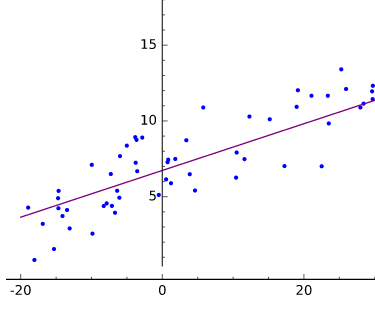
\includegraphics[scale=1.6]{img/regression.png}
		\caption{Linear regression plotted~\cite{tfidf}}
		\label{fig:regresion}
	\end{figure}
	\item \textit{Classification}: Classification is modeling based on delineating classes of output based on some set of input features. If regression gives us an outcome of "how much,” classification gives us an outcome of "what kind.”
	\item \textit{Clustering}: Clustering is an unsupervised learning technique that involves using a distance measure and iteratively moving similar items more closely together. At the end of the process, the items clustered most densely around $n$ centroids are considered to be classified in that group. $K-means$ clustering is one of the more famous variations of clustering in machine learning. 
\end{itemize} 

Furthermore, depending on the dataset the learning process can be carried out in two different ways:
\begin{itemize}
	\item \textit{Supervised learning:} \label{ml:super}The classifier is trained using a percentage of the total dataset while feeding the rest of the dataset to make predictions and to evaluate how good the classifier is. Particularly, this project will be using supervised learning.
	
	\item \textit{Unsupervised learning:} These algorithms base their learning properties on learning patterns present on the dataset. Unlike in supervised learning, there is no training and test dataset partition
\end{itemize}
Two major problems encountered in a~\ac{ml} application are underfitting and overfitting. These two problems appear due to the bias generated when training the model.\\
It turns out that depending on \textit{how much trained} the classifier is, it can make more assumptions than desired. A learned function that can perform well enough on unseen data points as well as on the training data is termed a generalizable function~\cite{gs}. A generalizable function is achieved through a generalizing fit. To get a proper fit, the function must not be biased, it must be perfectly balanced. 
\begin{itemize}
	\item \textit{Underfitting:}
	\begin{figure}
		\centering
		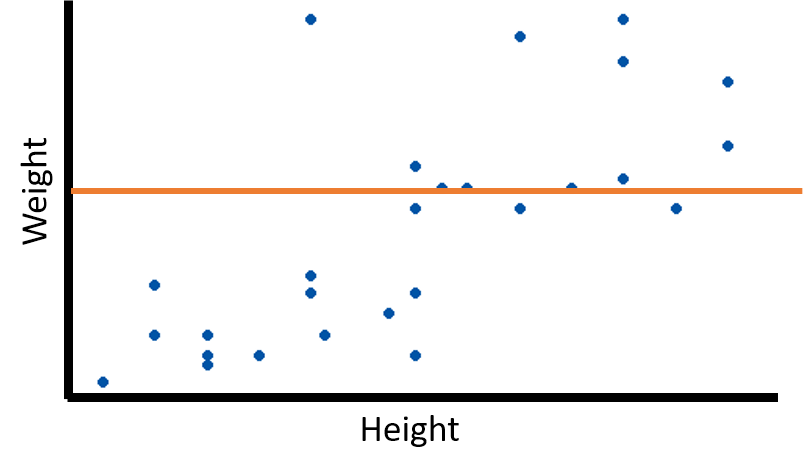
\includegraphics[scale=0.4]{img/underfit.png}
		\caption{Underfitting~\cite{gs}}
		\label{fig:underfit}
	\end{figure}
	\Cref{fig:underfit} shows that for any point in the diagram, the function always assigns the same predicted value. Solving the problem of underfitting means making the line approximate the data better.
	\item \textit{Overfitting:} 
	\begin{figure}
		\centering
		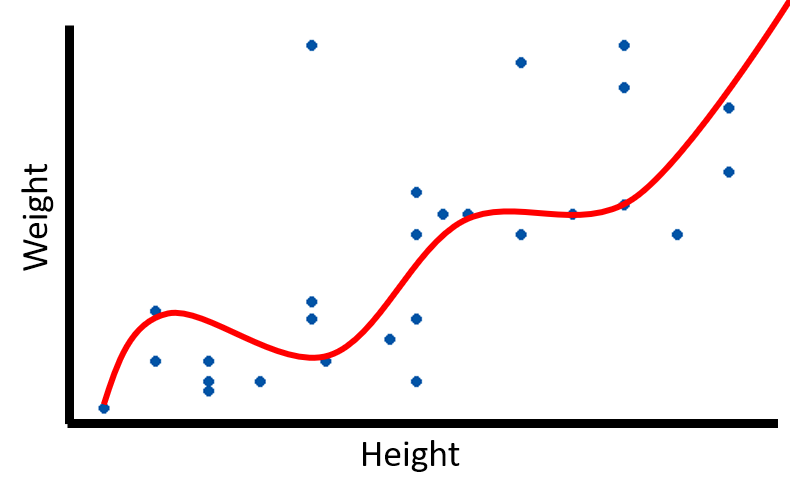
\includegraphics[scale=0.4]{img/overfit.png}
		\caption{Overfitting~\cite{gs}}
		\label{fig:overfit}
	\end{figure}
	\Cref{fig:overfit} shows that for any point in the diagram, the function performs very good. However, the function has become very inflexible and it will not perform good enough on new points. According to~\cite{tfidf}, overfitting can also be understood as a probable distribution of data. The training set of data that the line is being drawn through is just a sample of a larger unknown set, and the line which will be drawn needs to fit the larger set equally well if it is to have any predictive power. Therefore, it must be assumed that our sample is loosely representative of a larger set.
\end{itemize}
Another field of Artrificial Intelligence is~\ac{nlp}, which provides tools for analyzing and deriving meaning in human language. To do so,~\ac{nlp} provides a means to process lexical properties as well as syntactic recognition of the human language. However, human language can be rarely precise and ambiguous. Even though~\ac{nlp} has a very wide range of applications, such as automatic text summarizing, relationship extracting, stemming, sentiment analysis and more, it is a difficult problem to tackle in computer science.

\subsection{Sklearn}
\subsubsection{Definition}
Sklearn (a.k.a scikit-learn) is defined \footnote{http://scikit-learn.org/stable/} as a simple and efficient set of tools for data mining and data analysis. It is built on NumPy and SciPy. Sklearn will provide not only the classifiers needed for the pipeline but also meaningful tools.
\subsubsection{Application}
Sklearn has provided the following tools for this project:
\begin{itemize}
	\item \textit{Train and Test splitting}: This method is responsible for splitting the main dataset into two parts, one for training the model and the other one for testing the model. It is a very common~\ac{ml} technique. In addition, the testing set will later be used to compute parameters such as accuracy and f1 score. More information on accuracy and f1 score can be found in \cref{sec:score}.
	\item \textit{Pipeline}: A pipeline is a set of procedures connected in series, one after the other where the output of one process is the input to the next~\cite{pipeline1}. Image~\ref{fig:pipeline}\footnote{\url{https://www.slideshare.net/databricks/dataframes-and-pipelines}} represents the idea of a pipeline, though it does not resemble exactly this projects' pipeline.
	\item \textit{\acl{tfidf}}: The~\acf{tfidf} is used for every word. It contains two parts; the \textit{if} part, which represents the word frequency and the \textit{idf} part, which represents inverse document frequency~\cite{tfidf1}. This term represents a words' weight in a text.
	\item \textit{Count Vectorizer}: The algorithm consists of representing a token by considering how many times it appears in a text~\cite{countvect1}. It basically counts the vocabulary and generates a dictionary which can later be fed into a pipeline, like in this project.
	\item \textit{\acl{nb}}: A multinomial distribution useful to model feature vectors where each value represents a number of occurrences of a term (or its relative frequency)~\cite{countvect1}.
	\item \textit{\acl{svm}}: Given a set of training examples, each marked as belonging to one or the other of two categories, a \acf{svm} training algorithm builds a model that assigns new examples to one category or the other, making it a non-probabilistic binary linear classifier\footnote{\url{https://en.wikipedia.org/wiki/Support_vector_machine}}.
	\item \textit{\acl{knn}}: Is a non-generalized~\ac{ml} algorithm that computes distances from one point to all the training dataset points and chooses the $k$ nearest points~\cite{countvect1}.The KNeighbors classifier has been fed into the pipeline as input.
	\item \textit{\acl{lr} classifier}: Is analogous to multiple linear regression, except the outcome is binary. Various transformations are employed to convert the problem to one in which a linear model can be fit~\cite{lr1}.
\end{itemize}

\begin{figure}
	\centering
	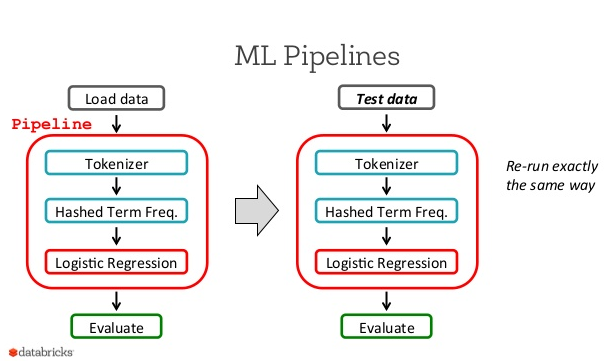
\includegraphics[width=\linewidth]{img/pipeline1.png}
	\caption{A Pipeline.~\cite{pipeline}}
	\label{fig:pipeline}
\end{figure}

All the methods illustrated above are widely explained altogether with an implementation clarification in~\cref{sec:clasif}.
\section{Senpy}
Senpy~\cite{senpy} is a framework for text analysis using linked data. It aims at providing a framework where analysis modules can be easily integrated as plugins and, at the same time, provides the core functionalities (data validation, user interaction, logging, etc).

\subsection{Architecture}
Senpy introduces a modular and dynamic architecture which allows implementing different algorithms in an extensible way while offering a common interface and offering common services that facilitate development, so developers can focus on implementing new and better algorithms.\par
To do so, the architecture consists of two main modules:
\begin{itemize}
	\item Senpy core: Building block of the service.
	\item Senpy plugins: Analysis algorithms.
\end{itemize}
\begin{figure}
	\hspace{-2.1cm}
	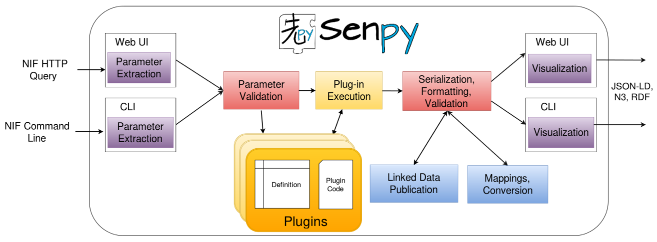
\includegraphics[scale=0.85]{img/senpy_architecture.png}
	\caption{Senpy's Architecture~\cite{senpy}}
	\label{fig:senpyarch}
\end{figure}
\Cref{fig:senpyarch} depicts a simplified version of the processes involved in Senpy analysis framework.

\section{Bitter}
\label{sec:bitter}
In order to download the Tweets which integrate partially the dataset, the tool bitter was used. Bitter is able to automate several actions (e.g. downloading Tweets) by using a Python wrapper over Twitter which adds support for several Twitter API actions~\footnote{https://github.com/balkian/bitter}.\\
Bitter could be used after installing it and running commands on the UNIX terminal.
\subsection{Architecture}
\Cref{fig:bitter} explains how was bitter used in this project. On the left, the reader can see the information provided to the bitter tool. The configuration file is needed to download the tweets, otherwise, nothing will be downloaded. The file contains the user credentials for accessing the Twitter database.\\ The tweet id file is a \textit{.csv} database containing in one column the desired tweets. Finally, bitter will download in \textit{.json} format all the tweets in the indicated folder (indicated on the command). For those tweets that, by any reason, could not be downloaded, a folder named \textit{error} will be created containing the tweet ids that failed.
\begin{figure}
	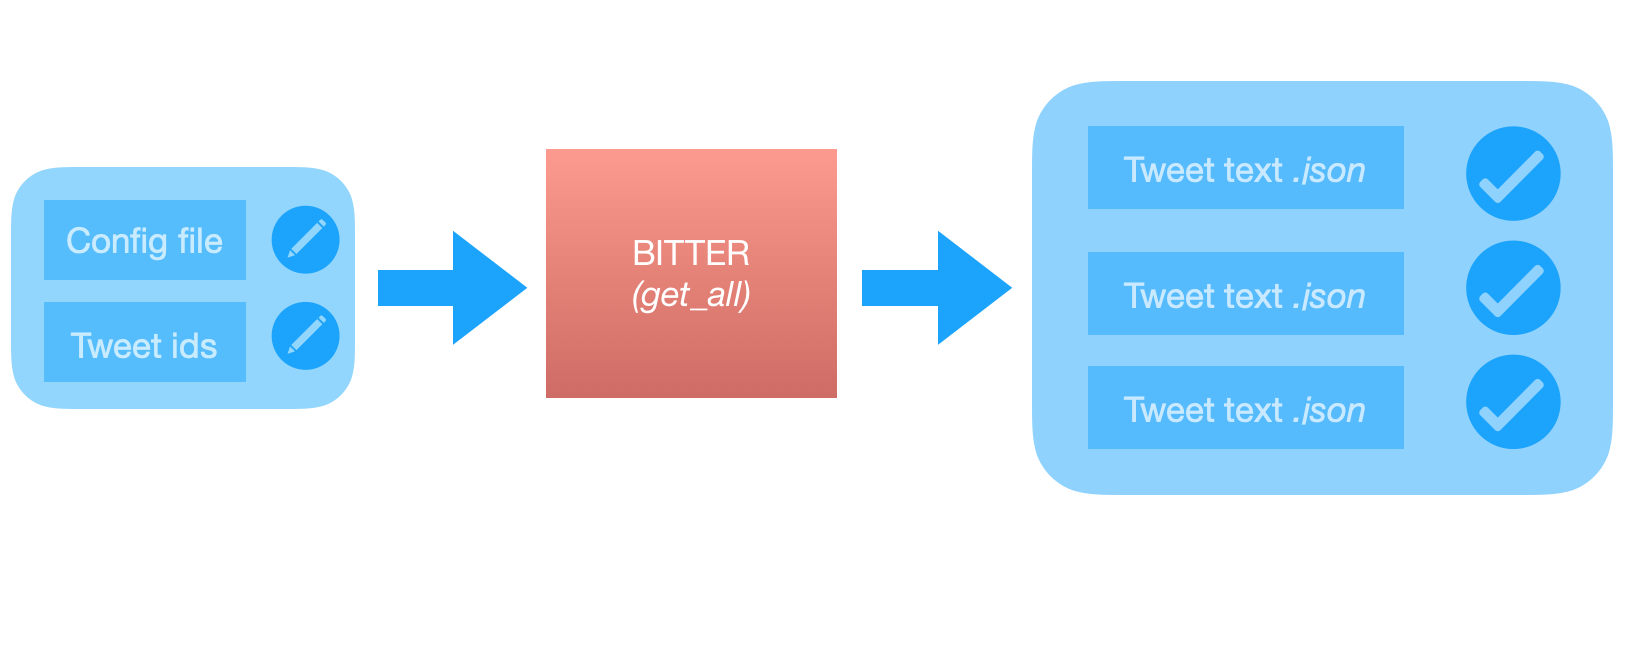
\includegraphics[width=\linewidth]{img/bitter.png}
	\caption{Bitter Architecture}
	\label{fig:bitter}
\end{figure}
\section{Elasticsearch}
Elasticsearch is a highly scalable open source search engine with a very powerful analytical engine. The data stored in Elasticsearch is \ac{json} formatted. The primary way of interacting with Elasticsearch is via \textbf{REST API}~\cite{elastic1}. The most powerful tool that Elasticsearch provides is indexing. Indexing becomes a very important task when dealing with lots of amount of data, in this case, with many tweets.
\subsection{Architecture}
All data stored in Apache Lucene's data is stored in \textit{inverted index}. This means that the data is being transformed. The process of transforming data is called analysis, which relies in two basic pillars: \textbf{tokenizing} and \textbf{normalizing}. The normalizing step is mandatory to make the tokens readable. Inverted index processes are performed by analyzers. An analyzer is composed of a tokenizer and one or more token filters. During the indexing time, when Elasticsearch processes a field that must be indexed, it checks whether an analyzer is defined in several levels~\cite{elastic1}.\\
When it comes to indices, Elasticsearch uses shards and replicas in order to distribute data around the cluster.\\
Elasticsearch distributes the shards by performing a process called \textit{sharding}. The indices (or index) are called shards and Elasticsearch automatically manages the shards, like a low-level working unit.
\begin{figure}
	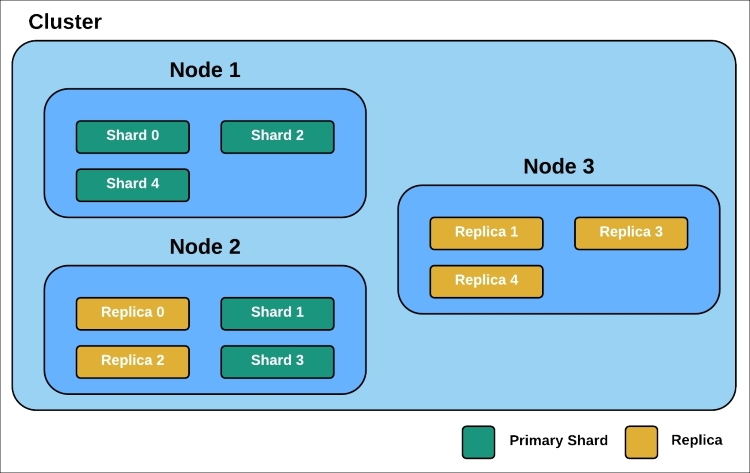
\includegraphics[width=\linewidth]{img/elasticsearch.jpeg}
	\caption{Elasticsearch~\cite{elastic3}}
	\label{fig:elastic1}
\end{figure}
The most common terms used in Elasticsearch are:
\begin{itemize}
	\item \textit{Node}: An instance of Elasticsearch running on a machine.
	\item \textit{Cluster}: The name under which one or more nodes are connected.
	\item \textit{Document}: A \ac{json} object containing the actual data in key-value pairs.
	\item \textit{Index}: Logical namespace in which Elasticsearch stores data.
	\item \textit{Doc types}: A class of similar documents. A type consists of a name and a mapping.
	\item \textit{Shard}: Containers which can be stored on a single node or multiple nodes. A  shard can be either primary or secondary. A primary shard is the one where all the operations that change the index are directed. A secondary shard is the one that contains duplicate data of the primary shard and helps in quickly searching the data as well as for high availability; in a case where the machine that holds the primary shard goes down, then the secondary shard becomes the primary automatically.
	\item \textit{Replica}: Duplicate copy of the data living in a shard for high availability.
\end{itemize}
Finally, as mentioned before, Elasticsearch can be related to a traditional database managing system. This is depicted in~\Cref{fig:elastic2}.
\begin{figure}
	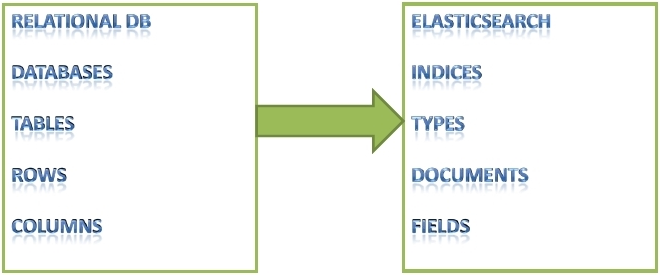
\includegraphics[scale=0.65]{img/elastic_1.png}
	\caption{Elasticsearch and a Database~\cite{elastic1}.}
	\label{fig:elastic2}
\end{figure}
\section{Pickle}
The pickle module makes it possible to store an object in a file in a standard format for later use by the same or a different program. The stored can be any type of object as long as it does not require an operating system resource such as a file handle or network socket~\cite{pickle}.\\
Pickle is very useful for using an already trained classifier in different modules.




